% Name: Standing wave
% Description: The third harmonic on a string fixed at both ends: the wave at several moments inside its envelope, with nodes N where it never moves and antinodes A where it swings most.
% Tags: standing wave, harmonics, nodes, antinodes, string

\usetikzlibrary{patterns}

\begin{tikzpicture}[every node/.style={font=\small}]
  % y = 1.2 sin(3 pi x / 8) cos(wt) on 0 <= x <= 8: nodes at 0, 8/3, 16/3, and 8, antinodes at 4/3, 4, and 20/3.
  \fill[pattern=north east lines, pattern color=gray] (-0.25,-1.6) rectangle (0,1.6) (8,-1.6) rectangle (8.25,1.6);
  \draw[thick] (0,-1.6) -- (0,1.6) (8,-1.6) -- (8,1.6);
  \draw[dashed, gray] (0,0) -- (8,0);
  \foreach \c in {0.5,-0.5} \draw[blue!50, domain=0:8, samples=100, smooth] plot (\x, {\c*1.2*sin(67.5*\x)});
  \foreach \c in {1,-1} \draw[very thick, blue!70!black, domain=0:8, samples=100, smooth] plot (\x, {\c*1.2*sin(67.5*\x)});
  \foreach \x in {0,2.667,5.333,8} \fill[red!70!black] (\x,0) circle (2pt);
  \foreach \x in {0.2,2.667,5.333,7.8} \node[red!70!black] at (\x,-1.35) {N};
  \foreach \x in {1.333,4,6.667} \node[above, green!40!black] at (\x,1.25) {A};
  \draw[|<->|, gray!40!black] (0,-2) -- node[below] {$L = \tfrac{3}{2}\lambda$} (8,-2);
\end{tikzpicture}
